\documentclass[11pt]{article}

\usepackage[T1]{fontenc}
\usepackage{times}
\usepackage{latexsym}
\usepackage{microtype}
\usepackage{booktabs}
\usepackage{graphicx}
\usepackage{amsmath}
\usepackage[margin=0.85in]{geometry}
\usepackage[round]{natbib}
\usepackage[hidelinks]{hyperref}

% Keep compact subheadings visually distinct.
% A positive after-skip makes paragraph headings block-level, bold, and left-aligned.
\makeatletter
\renewcommand\paragraph{\@startsection{paragraph}{4}{\z@}{1.25ex plus
   0.4ex minus .2ex}{0.25ex}{\normalsize\bfseries\raggedright}}
\makeatother

\title{Perplexity and Fluency after Continual Chinese Adaptation of a 42M-Parameter Llama-2}

\author{Cand1eLight}

\date{}
\begin{document}
\maketitle

\begin{abstract}
I evaluate English generation, cross-lingual perplexity, and Chinese continual pre-training
with a 41.69M-parameter Llama-2-style model trained on TinyStories. The generation study
contains 72 continuations from four prompt types and six decoding settings. Beam search is
stable but repeats the same output across seeds. High-temperature nucleus sampling produces
more varied text, with weaker causal links in several samples. On the official test sets,
the base model obtains token-weighted perplexity (PPL) 3.14 in English and 117,885 in Chinese.
After 1,200 Chinese updates, Chinese PPL falls to 4.80 and English PPL rises to 7.07. Adding
1,000 English rehearsal stories to the 10,000 Chinese stories gives Chinese PPL 5.05 and
English PPL 2.86. The generated Chinese improves at the phrase level, although longer
stories still contain changes in character identity and implausible events.
\end{abstract}

\section{Introduction}

TinyStories shows that very small language models can learn fluent, multi-paragraph
English when their training domain and vocabulary are tightly controlled
\citep{eldan2023tinystories}. The same specialization creates an informative continual
learning problem: can an English model acquire Chinese without destroying what it already
knows? I investigate this with a 42M Llama-2-style causal model
\citep{touvron2023llama,karpathyTinyLlamas}.

I compare six decoding settings across four prompt types, then evaluate the same checkpoint
on English, Chinese, and Portuguese with matched token budgets. Continual training holds the
update count and optimizer settings fixed while varying the learning rate and corpus
composition. The final run adds a small English replay sample to test whether it can preserve
the original language while the model learns Chinese.

\section{Experimental Setup}

\paragraph{Data}
I use the supplied local checkpoint and official archive: 10,000/500/1,000 Chinese
train/development/test stories, 1,000 English test stories, and matched Portuguese splits.
The course archive contains no English training split, so the replay condition uses 1,000
separately sampled TinyStories training stories \citep{gabrui2024multilingual}. Seed 7021,
source labels, and SHA-256 hashes are recorded. All reported evaluation and training results
use the supplied checkpoint and official test files.

\begin{table}[t]
\centering
\footnotesize
\setlength{\tabcolsep}{3pt}
\begin{tabular}{@{}lrrr@{}}
\toprule
Split & Docs & Median chars & Mean tokens \\
\midrule
Chinese train & 10,000 & 239 & 405.1 \\
Chinese dev & 500 & 240 & 401.0 \\
Chinese test & 1,000 & 242 & 408.8 \\
English test & 1,000 & 738 & 206.1 \\
Portuguese test & 1,000 & 703 & 256.3 \\
\bottomrule
\end{tabular}
\caption{Corpus statistics under the unchanged base tokenizer.}
\label{tab:data}
\end{table}

\paragraph{Model and Tokenization}
The supplied checkpoint contains 41,689,600 parameters and uses the original 32K
SentencePiece tokenizer. No vocabulary items are added. Chinese requires 1.595 tokens per
visible character, compared with 0.267 for English, a 5.95$\times$ fragmentation penalty.
Thus the same 256-token block covers much less visible Chinese context. This agrees with
prior findings that tokenizer quality can materially change multilingual model performance
\citep{rust2021good}.

Stories are separated by EOS and packed into 256-token blocks. Evaluation uses the same
128 blocks (32,640 predicted tokens) for every checkpoint. I accumulate token-weighted
negative log-likelihood $L$ and report $\exp(L)$. Packing eliminates padding as a confound;
using fixed evaluation blocks makes all model comparisons paired.

\section{English Generation}

The prompt set contains (i) a conventional story opening, (ii) dialogue, (iii) an explicit
``no magic'' constraint, and (iv) a counterfactual village. Each is decoded three times per
setting. Greedy and four-beam search serve as deterministic controls. Sampling settings vary
temperature, top-$k$, and nucleus probability. I report corpus-level Distinct-2, within-text
repeated four-gram fraction, and the fraction of unique first sentences.

\begin{table}[t]
\centering
\footnotesize
\setlength{\tabcolsep}{2.5pt}
\begin{tabular}{@{}lrrr@{}}
\toprule
Decoder & Dist-2 $\uparrow$ & Rep-4 $\downarrow$ & Unique open. \\
\midrule
Greedy & .252 & .0176 & .333 \\
Beam-4 & .270 & .0083 & .333 \\
Low temp. ($.45$) & .678 & .0210 & 1.000 \\
Top-$k$ 50 & .725 & .0091 & 1.000 \\
Nucleus $p=.90$ & .712 & .0082 & 1.000 \\
High temp. ($p=.95$) & \textbf{.874} & \textbf{.0008} & 1.000 \\
\bottomrule
\end{tabular}
\caption{Decoding statistics from 12 outputs per setting.}
\label{tab:decode}
\end{table}

\begin{figure}[t]
\centering
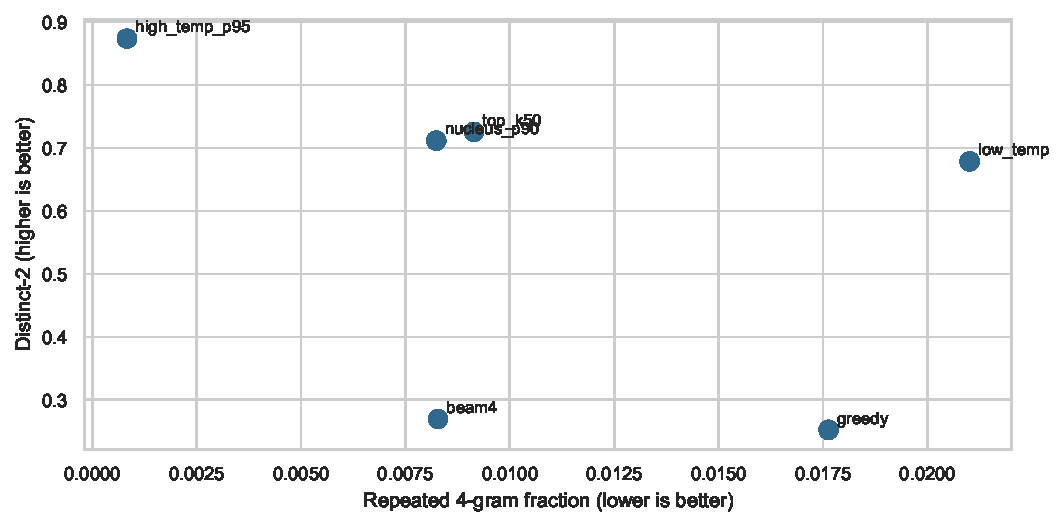
\includegraphics[width=\columnwidth]{../figures/decoding_frontier.pdf}
\caption{Diversity and repetition across all 12 outputs for each decoding setting.}
\label{fig:decode}
\end{figure}

Beam search produced a clean key-and-door narrative, but its three runs for each prompt
were identical. High-temperature nucleus sampling achieved the best lexical diversity and
lowest exact repetition. Case inspection also found abrupt entity changes and weaker causal
links. Top-$k$ 50 gave the most useful balance in this experiment, with high diversity and
fewer serious coherence failures. None of the 72 samples emitted EOS within 128 new tokens.
The fixed cutoff determines their similar lengths and prevents this run from measuring
learned stopping behavior.

Prompt form also mattered. Dialogue openings were usually continued as dialogue, while the
instruction-like constraint was often treated as part of the story. Its behavior follows the
TinyStories continuation distribution, so instruction-like prompts do not reliably impose
negative constraints on this base model.

\section{Perplexity and Continual Training}

The base model's fixed-budget English PPL is 3.14. Chinese test PPL is 117,885.17
(development: 111,207.01), over four orders of magnitude higher; Portuguese is also poor
at 26,522.53. A Chinese prompt immediately elicits English before adaptation. The scale of
this gap and the tokenizer fragmentation show that language mismatch is the main problem.

I tune learning rate with identical 80-update runs. All runs use AdamW, batch size 8,
two-step gradient accumulation (4,096 tokens/update), 6\% linear warm-up, cosine decay,
weight decay 0.1, gradient clipping at 1.0, and bfloat16. Table~\ref{tab:lr} selects
$2\times10^{-4}$ by Chinese development PPL; the larger rate converges quickly but is
slightly worse under the same budget.

\begin{table}[t]
\centering
\small
\begin{tabular}{rrr}
\toprule
Learning rate & Dev PPL & Time (s) \\
\midrule
$5\times10^{-5}$ & 412.55 & 12.4 \\
$2\times10^{-4}$ & \textbf{151.27} & 12.8 \\
$8\times10^{-4}$ & 154.39 & 12.5 \\
\bottomrule
\end{tabular}
\caption{Equal-budget learning-rate sweep (80 updates each).}
\label{tab:lr}
\end{table}

Two final runs use 1,200 updates. The Chinese-only corpus is compared with a shuffled mix of
10,000 Chinese and 1,000 English rehearsal stories. Rehearsal follows the general continual
learning idea of preserving representative old-task examples \citep{lopezpaz2017gem}; it
adds no model parameters and both conditions receive the same optimizer-step budget.

\begin{table}[t]
\centering
\footnotesize
\setlength{\tabcolsep}{2.2pt}
\begin{tabular}{@{}lrrrr@{}}
\toprule
& \multicolumn{2}{c}{Fixed-token} & \multicolumn{2}{c}{Document mean} \\
Checkpoint & ZH & EN & ZH & EN \\
\midrule
Base & 117,885.17 & 3.14 & 76,898.29 & 3.53 \\
Chinese-only & \textbf{4.80} & 7.07 & \textbf{4.86} & 8.84 \\
ZH+EN rehearsal & 5.05 & \textbf{2.86} & 5.77 & \textbf{4.38} \\
\bottomrule
\end{tabular}
\caption{Official test PPL. Fixed-token uses 32,640 predictions; document mean follows
\texttt{compute\_ppl} with a 512-token cap.}
\label{tab:ppl}
\end{table}

\begin{figure}[t]
\centering
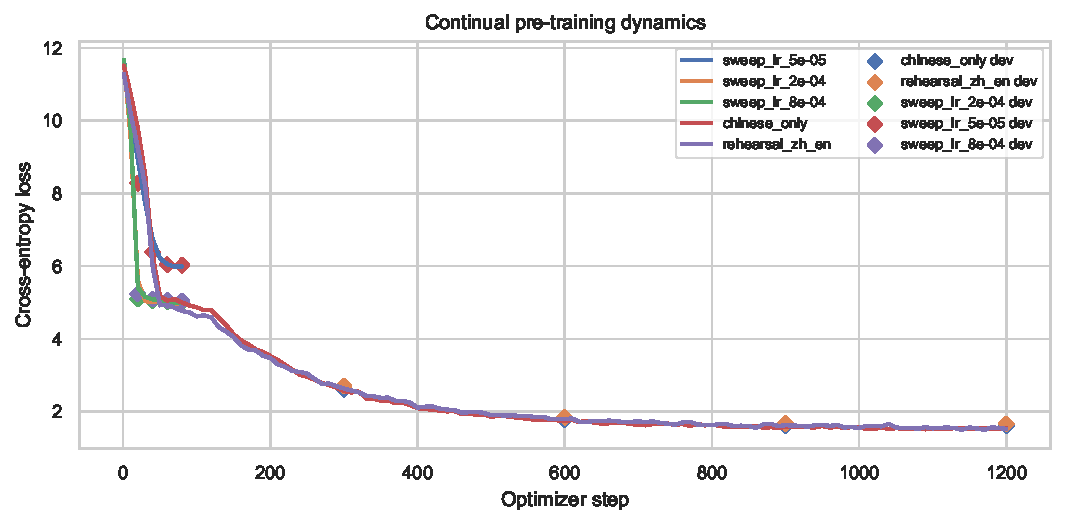
\includegraphics[width=\columnwidth]{../figures/training_curves.pdf}
\caption{Training loss (lines) and fixed Chinese development loss (diamonds). Curves include
the sweep and both final runs; logs are recorded every 10 updates.}
\label{fig:training}
\end{figure}

Chinese-only training reduces fixed-budget target PPL by 24,555$\times$, while English
becomes 2.25$\times$ worse. Portuguese PPL also rises to 214,567, which shows that the update
causes language-specific interference. With rehearsal, Chinese PPL is 5.1\% higher than the
Chinese-only result and English PPL is 59.6\% lower. Fixed-token English PPL is below the base
result, while document-mean English PPL remains above it. The document mean gives every story
equal weight and is more affected by short, difficult examples. Fixed packing gives every
predicted token equal weight. Both metrics show that rehearsal preserves English better than
Chinese-only training.

\section{Perplexity and Generated Story Quality}

After adaptation, 72--90\% of visible generated characters are Chinese. The outputs also
acquire Chinese punctuation, dialogue, names, and paragraph structure, and some short clauses
read naturally. Across longer passages, characters change identity, objects receive
incompatible actions, and several endings stop mid-byte at the fixed cutoff. The rehearsal
run shows the same pattern.

Teacher-forced likelihood rewards likely local continuations even when errors accumulate
during free generation. The byte-heavy tokenizer can also make familiar short fragments easy
to predict while reducing the amount of visible context in each block. Model size and the
single packed training epoch impose further limits. In this experiment, PPL tracks local
adaptation more reliably than overall story quality, so the generations need a separate
qualitative or human evaluation.

\section{Conclusion}

The decoding comparison shows a clear trade-off between varied wording and stable story
structure. Top-$k$ 50 gives the best balance among the tested settings. Continual training
closes most of the Chinese likelihood gap, but Chinese-only training damages English and
Portuguese performance. A 9.1\% story-level English rehearsal share keeps English close to
its original level for a 5.1\% increase in Chinese PPL. This makes the rehearsal checkpoint
the better choice when both Chinese adaptation and English retention matter. Future work
should test a Chinese-aware tokenizer, collect human ratings from multiple assessors, and
use longer generations to measure EOS behavior.

{\small
\setlength{\bibsep}{0pt plus 0.3ex}
\clearpage
\bibliographystyle{plainnat}
\bibliography{references}
}

\end{document}
